\subsection{Ca sử dụng xem chi tiết ảnh}

\vspace{0.5cm}

\noindent 
\begin{tabularx}{\linewidth}{| l | X |} 
\hline 
\textbf{Mô tả} & Người dùng xem thông tin chi tiết của ảnh \\
\hline 
\textbf{Luồng cơ bản} & 1. Người dùng chọn ảnh muốn xem thông tin trong màn hình thư viện. \newline
                       2. Hệ thống hiển thị ảnh ở chế độ toàn màn hình cùng thanh công cụ.\newline
                       3. Người dùng bấm nút xem thêm thông tin ảnh. \newline
                       4. Hệ thống hiển thị các thông tin của ảnh. Bao gồm: tên ảnh, album ảnh thuộc về, kich cỡ, caption ảnh, ngày tải lên, khuôn mặt trong bức ảnh, các nhãn và địa điểm chụp. \\
\hline 
\textbf{Tiền điều kiện} & - Người dùng đăng ký / đăng nhập tài khoản thành công và hoàn thành điền form thông tin cơ bản. \newline
                        - Người dùng đã tải ít nhất 1 ảnh lên thư viện. \\
\hline 
\textbf{Hậu điều kiện} & - Hệ thống hiển thị các thông tin ảnh chi tiết cho người dùng. \\
\hline 
\textbf{Yêu cầu phi chức năng} & Hệ thống truy vấn các thông tin của ảnh không quá 2s. \\
\hline 
\end{tabularx}

\vspace{0.8cm}

\noindent 
\begin{tabular}{| c | c |}
    \hline
    \textbf{Biểu đồ hoạt động} & \textbf{Quan hệ} \\ 
    \hline
    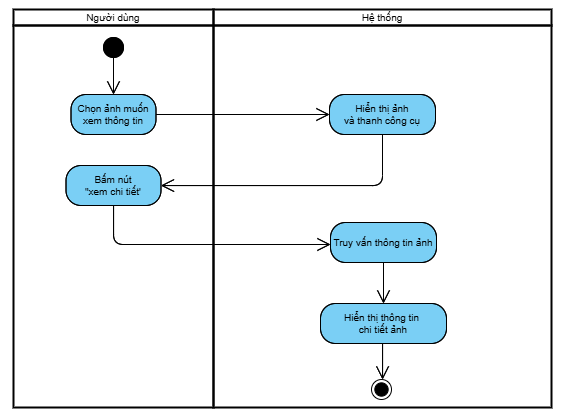
\includegraphics[width=0.6\linewidth]{figures/c3/3-3-5-activity-diagram.png} 
    & 
    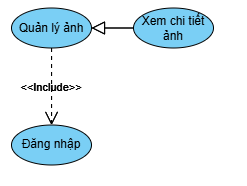
\includegraphics[width=0.35\linewidth]{figures/c3/3-3-5-relationship.png} \\ 
    \hline
\end{tabular}

\begin{figure}[H]
    \centering  
    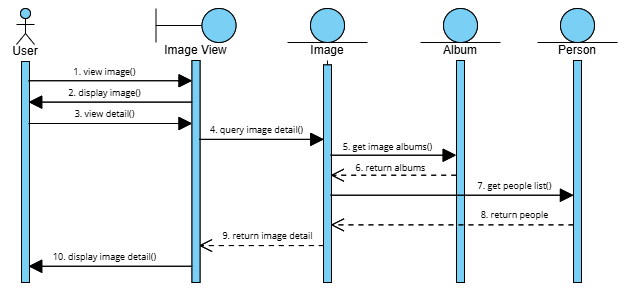
\includegraphics[width=1\textwidth]{figures/c3/3-3-5-sequence-diagram.png}
    \caption{Biểu đồ tuần tự ca sử dụng xem chi tiết ảnh.}
    \label{fig:3-3-5-sequence-diagram}
\end{figure}
